\documentclass[12pt,a4paper,english,titlepage,oneside]{scrbook}
% ***** BEGIN OF THE LATEX PREAMBLE *****

\usepackage{softeng,tabularx}
\usepackage[table]{xcolor}
\usepackage{amssymb,wasysym}
\definecolor{lightgray}{gray}{0.9}
\definecolor{lightblue}{RGB}{190,190,220}
\definecolor{lightgreen}{RGB}{190,220,220}
\definecolor{lightred}{RGB}{220,190,190}
\definecolor{heavyred}{RGB}{220,140,140}

% Here we define the title of the current thesis in an appropriate variable.
\newcommand{\worktitle}{Agile Startups}
% Here we can define a subtitle for the work. If there is no subtitle let this variable empty.
%\newcommand{\worksubtitle}{}
% otherwise you can set any subtitle you want, event long ones by breaking the lines manually:
\newcommand{\worksubtitle}{Comparision of Agile Methodololgy with the business canvas model}
			   
% This is the name of the author
\newcommand{\theauthor}{Johannes Eifert, Jean-Daniel Mathieu, Oleg Telegin, Daria XYZ}

% This command defines the type of the work: Master Thesis / Bachelor Thesis
\newcommand{\worktype}{Semester Work}

% Date of the end (submission) of the work.
\newcommand{\workdateyear}{2013}
\newcommand{\workdatemonth}{Mars}

% English: Thesis supervisors
% French: Supervis� par
% German: Unter der Aufssicht von
\newcommand{\supervisorslabel}{Thesis supervisors}

\newcommand{\worksupervisors}{
    Dr. Jean \textsc{Hennebert} \\
    University of Fribourg, Switzerland    
    % if there are other supervisor from other organisations, add them like this
    % \vspace{0.2cm}
    % Dr. Olivier \textsc{Liechti}\\
    % Sun Microsystems Inc.\\
}

% Set the titlepage footer according to the language of you report (E nglish, F rancais or D eutsch)
\newcommand{\titlepagefooter}{\titlepagefooterE}
%\newcommand{\titlepagefooter}{\titlepagefooterD}
%\newcommand{\titlepagefooter}{\titlepagefooterF}


% Here you define the labels of figures, tables, listings...
% English: Figure, Table, Listing (default)
% German: Abbildung, Tabelle, Listing
% French: Figure, Table, Listing
\renewcommand{\figurename}{Figure}
\renewcommand{\tablename}{Table}
\renewcommand{\lstlistingname}{Code extract} % default = Listing



% If you are still working on a draft version, this command prints a little slight note on the top left corner of each page.
% Comment this line when you have a final version.
\reviewtimetoday{\today}{* Draft Version *}

% Let us set the path where all the figures have to be.
\graphicspath{{./figures/}}

% The following command avoids the indentation of the first sentence of each paragraph.
\parindent=0in

% The following command sets the header and footer style of the pages.
\pagestyle{fancy}

% The web resources are references in a bibliography apart.
%\newcites{web}{Referenced Web Ressources}

% It is not mandatory (but suitable) to make an index. If you do not build an index: comment the line below!
% building the idx index file. This file is then to be compiled with %
% makeindex in the command line %
\usepackage{makeidx} \makeindex

% XML LstListing language settings
\definecolor{gray}{rgb}{0.4,0.4,0.4}
\definecolor{darkblue}{rgb}{0.0,0.0,0.6}
\definecolor{cyan}{rgb}{0.0,0.6,0.6}

\lstset{
  basicstyle=\ttfamily\footnotesize,
  columns=fullflexible,
  showstringspaces=false,
  commentstyle=\color{gray}\upshape
}

\lstdefinelanguage{XML}
{
  morestring=[b]",
  morestring=[s]{>}{<},
  morecomment=[s]{<?}{?>},
  stringstyle=\color{black},
  identifierstyle=\color{darkblue},
  keywordstyle=\color{cyan},
  morekeywords={xmlns,version,type}% list your attributes here
}


% ***** END OF THE LATEX PREAMBLE *****

% ***** BEGIN OF THE DOCUMENT *****
% ----- BEGIN OF THE FRONT STUFF -----
\begin{document}
% This line generates mini table of contents (tocs) at the beginning of each chapter, [e] for empty title.
\dominitoc[e] 
\pagestyle{empty}

% Here we include the titlepage.
\begin{titlepage}
\begin{center}
%    Department of Informatics\\
%    University of Fribourg, Switzerland\\
%    \apath{http://diuf.unifr.ch/}\\

    \vspace*{1.5cm}

    \begin{huge}
        {\sf \worktitle \\}
    \end{huge}
    \vspace{0.4cm}%
    \ifthenelse{\equal{\worksubtitle}{}}{}{\begin{Large} {\sf \worksubtitle} \end{Large}}%

    %Here you can put your own project logo, if you have one
    %\vspace{1cm}
    %\includegraphics[height=1.5cm]{figures/projectLogo.eps}
   
    ~
    \\[2.0cm]

    
     \begin{normalsize}
	{\textsc{\worktype}}\\
     \end{normalsize}
    ~
    \\[1.5cm]
     \begin{LARGE}
	{\textsc{\theauthor}}\\
        \vspace{0.2cm}
     \end{LARGE}
     \begin{large}
        {\workdate}
     \end{large}
    
    ~
    \\[4.0cm]
    
    \textbf{\supervisorslabel}:\\
    \vspace{0.2cm}
    \worksupervisors
    \vspace*{1.5cm}
    ~
    \\[1.0cm]

    \titlepagefooter

\end{center}

\end{titlepage}


% The first pages are numbered in roman style.
\pagenumbering{roman}

% You can set a quote or thought or dedication or whatever you want on this page.
% If you do not want to, simply comment the the three lines below!
%\section*{}  % Here you can put an inspiring quote or a special dedication...

\begin{flushright}
\vspace{1.5cm}
\squote{We make a living by what we get, we make a life by what we give.}\\
\vspace{0.2cm}
\textit{- Sir Winston Churchill}
\end{flushright}

% or a special dedication

%\vspace*{5cm}
%\begin{center}
%\textit{To my parents.}
%\end{center}



% If there is a diule/acknowledgements you can insert it here
%\chapter*{Acknowledgements}

bla bla bla

\pagestyle{headings} 

% Now we include the abstract of you work.
%\chapter*{Abstract}

\par{
The following work is a reproduction of the steps used to build a fully functional web service in a eHealth environment as a web of things. The final product is composed of two parts: a client and a server application.}
\par{The server is used to store and manipulate data that caregiver in a medical facility have to work with on a daily basis. It is designed towards accessibility and openness and allows access by any internet capable device, providing that the user is authenticated. }
\par{The client on the other hand is designed to facilitate daily work by presenting the stored data in a practical manner. Adding, modifying and removing data must be as intuitive as possible. }

% and keywords...

\vspace*{1cm}
\textbf{Keywords:} eHealth,Web of things, RESTful

% In order to have all references in your bibtex files figuring in the bibliorgraphy you can uncomment following lines.
% Otherwise, only the cited references will appear in your bibliography.
\nocite{*}
%\nociteweb{*}

\begin{spacing}{1.2}  % Environment for 1.2 line spacing for contents and lists

% Here comes the table of contents
% Setting the name of the table of contents
%\renewcommand{\contentsname}{Table of Contents}  % Original name = Contents
%\tableofcontents    % table of contents (.toc file) -- to rename title \renewcommand{\contentsname}{Table of Contents}

% Here comes the list of figures
%\listoffigures    % list of figures   (.lof file) -- to rename title \renewcommand{\listfigurename}{Figures}

% Here comes the list of tables
%\listoftables    % list of tables    (.lot file) -- to rename title \renewcommand{\listtablename}{Tables}

% Here comes the list of listings/code extracts
% Setting the name of the table of listings
%\renewcommand{\lstlistlistingname}{List of Code extracts}  % Original name = Listings
%\lstlistoflistings    % list of listings    (.lol file) -- to rename title \renewcommand{\listtablename}{Tables}

\end{spacing}  % Environment for 1.2 line spacing for contents and lists

% ----- END OF THE FRONT STUFF -----

% ----- BEGIN OF THE MAIN BODY OF THE DOCUMENT -----

% Page numbering will now be arabic.
\pagenumbering{arabic}

\addtolength{\parskip}{0.25\baselineskip} % paragraph spacing

\chapter{Abstract}
\par{
The following work is a comparison of the theories about the business canvas model and the agile methdology. 
}
\chapter{Introduction to Agile}
This chapter gives an overview over agile software development processes in general.\\

In the traditional software development there are many people working on the requirements of the future software. When this is done, the developers start to work on it. During this phase there is usually no feedback from either the product owner or future users. The developers work more or less on their own which usually results in a disaster. (Quelle: http://www.galorath.com/wp/software-project-failure-costs-billions-better-estimation-planning-can-help.php) According to blabla only 32 percent of the IT projects in were successful. This needs to be changed and agile methodologies are trying to do that by trying to produce something valuable instead of over-planning.

\section{The Agile Processes}
The agile software development processes work in iterations. These are repeated at least until the software is shippable. A very important aspect of the process is the fact that after each iteration there should be an increment of the project which has some value and would be shippable.

\subsection{Principles}
\cite{beck2001manifesto} lists principles of agile processes. A few of them are denoted in the following enumeration:
\begin{enumerate}
\item Our highest priority is to satisfy the customer through early and continuous delivery of valuable software.
\item Welcome changing requirements, even late in development. Agile processes harness change for the customer's competitive advantage. 
\item Deliver working software frequently, from a couple of weeks to a couple of months, with a preference to the shorter time-scale.
\item Business people and developers must work together daily throughout the project.
\item Build projects around motivated individuals. Give them the environment and support they need, and trust them to get the
job done.
\item The most efficient and effective method of conveying information to and within a development team is face–to–face conversation.
\item Working software is the primary measure of progress.
\item At regular intervals, the team reflects on how to become more effective, then tunes and adjusts its behaviour accordingly.
\end{enumerate}


\subsection{Limits}
According to \cite{turk2002limitations} the usage of the agile software development processes brings a few drawbacks and limitations:
\begin{enumerate}
\item Limited support for distributed development environments.
\item Limited support for subcontracting.
\item Limited support for building reusable artefacts.
\item Limited support for development involving large teams.
\item Limited support for developing large, complex software.
\item Limited support for developing safety-critical software.
\end{enumerate}
In chapter blabla we discuss if these limitations also apply to our agile start up process.

\cite{scrum_linda}
\chapter{Scrum}
\section{Introduction to Scrum}

\par{
Scrum is originally a tactic used in rugby. All players are gathered around the ball, holding each other and trying to be the first team to get the ball. Scrum is applied when an error was made or a ball was put out of game. The scrum methodology is an applied software team management philosophy following the same principle. It is agile and therefore an ideal example for an applied agile methodology. 
\par{
Scrum not only tries to avoid errors like the "tunnel development", "contract gaming", "squirrel burgers" or working with the "magic toolbox" but it also enforces a game like style in design and implementation of Software. A Scrum team is considered very transparent and flexible, giving always clear information about the current state of the development. 
}
\par{
Main goal is to generated measurable value increments after each step in the development of software, by minimizing the time between each working increment of the software.
}
\section{Scrum Principles and elements}
\subsection{Radiator, stories, backlog and sprints}
\par{
The center piece of scrum is a big chart showing the overview of all currently developed features. This chart is called the radiator while the features are called stories. A story is comparable to a specific feature. Each described as a use-case and containing an estimation in time or points for the completion. Those information are written on a post-it and put on the radiator. 
}
\par{
The radiator does not only show the current stories but all stories, whether they are completed, in progress or in the backlog. The radiator also contains a chart summing up the current points in progress, the points already used and the remaining points. This chart is called a burn-down diagram. This gives an always-up-to-date overview of the current state of the project and is visible to anyone working on the project. 
}
\par{
Another element are the sprints. They are time frames set to finish the next set of stories. Stories assigned to a project are stored in the sprint-backlog. All stories assigned to the team are stored in the product backlog. 
}
\begin{figure}[h!]
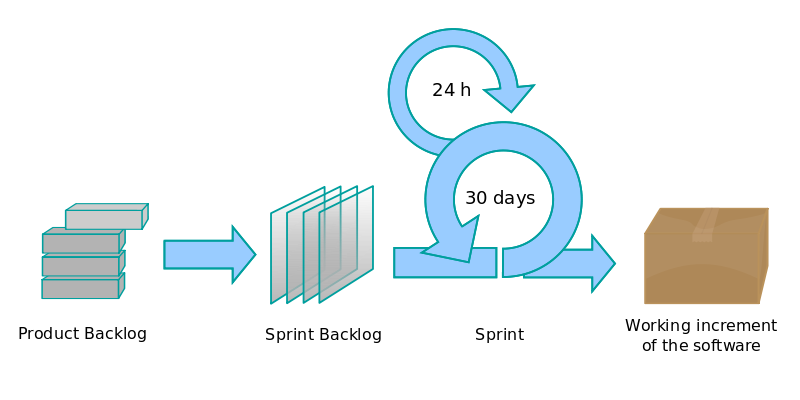
\includegraphics[width=\textwidth]{scrum_process.png}
\caption{\label{scrumproc}Illustration of the scrum process}
\end{figure}

\subsection{Roles}
\textbf{product-owner}
\par{
The most important role in Scrum is the product-owner. He is responsible to present new stories and priories them. He is the manager behind the backlog and directs the team to fulfill the goals set by the stakeholders. 
}
\\\\
\textbf{scrum-master}
\par{
Takes over the role of a mentor and guide to apply the scrum rules. He controls the teams and leads discussion and meetings. He is not to be confused with the product-owner as a scrum-master does not manage the team, but only leads it. He can be compared to the coach. A Scrum master protects the teams from any influence and helps focusing on the tasks ahead.
}
\\\\
\textbf{developer-team}
\par{
Of course every team needs grunts for the work. Developer take over the role as designer and developer. They follow instructions and are organized as teams. Each team focusing on the same stories.
}
\\\\
\textbf{stakeholders}
\par{
Stakeholders are the customers. They provide feedback to the product-owner and provide the income. They are only involved in the sprint meetings. 
}
\\\\
\textbf{management}
\par{
The management has no special function but to provide stakeholders (Marketing) and deliver a work environment for the developer teams (Facility Manager, HR Manager). 
}
\subsection{Meetings}
\subsubsection{Daily Scrums}
\par{
Daily meeting used to check on work progress. Therefore it is discussed what changed since last meeting and what is up ahead. Those meetings are timeboxed to 15 minutes.
}
\subsubsection{Backlog grooming}
\par{
A meeting done during a sprint. The current stories are updated and new stories are optimized using techniques like planning poker. After such a meeting the backlog is re estimated providing sharper estimation of project state.
}
\subsubsection{Scrum of Scrums}
\par{
Meeting of team or clusters of teams to discuss overlapping stories or common work. Usually after a daily scrum.
}
\subsubsection{Sprint planning meeting}
\par{
Meeting before the start of a sprint to fix the backlog.
}
\subsubsection{End of cycle}
\par{
Meeting at the end of a sprint to discuss the sprint in retrospective. This can be seen as an after action review or a debriefing. 
}
% \include{chapters/chapter1}

%\include{chapters/chapter2}

%\include{chapters/conclusion}

% ----- END OF THE MAIN BODY OF THE DOCUMENT -----

% ----- BEGIN OF THE APPENDICES -----
\appendix

% First we enumerate the most often used acronyms
%\chapter{Common Acronyms}\label{acronyms}

% You have to sort them manually

\begin{acronym}
\acro{API}  {Application Programming Interface}
\end{acronym}

\begin{acronym}
\acro{ASCII}  {American Standard Code for Information Interchange}
\end{acronym}

\begin{acronym}
\acro{CORBA}  {Common Object Request Broker Architecture}
\end{acronym}

\begin{acronym}
\acro{CSCW}  {Computer Supported Collaborative Work}
\end{acronym}

\begin{acronym}
\acro{CVS}  {Concurrent Versions System}
\end{acronym}

\begin{acronym}
\acro{EJB}  {Enterprise Java Beans}
\end{acronym}

\begin{acronym}
\acro{FTP}  {File Transfer Protocol}
\end{acronym}

\begin{acronym}
\acro{HTML}  {Hypertext Markup Language}
\end{acronym}

\begin{acronym}
\acro{IDE}  {Integrated Development Environment}
\end{acronym}

\begin{acronym}
\acro{IRC}  {Internet Relay Chat}
\end{acronym}

\begin{acronym}
\acro{J2EE}  {Java 2 Platform, Enterprise Edition}
\end{acronym}

\begin{acronym}
\acro{NAT}  {Network Address Translation}
\end{acronym}

\begin{acronym}
\acro{OCL}  {Object Constraint Language}
\end{acronym}

\begin{acronym}
\acro{OCR}  {Optical Character Recognition}
\end{acronym}

\begin{acronym}
\acro{OMG}  {Object Management Group}
\end{acronym}

\begin{acronym}
\acro{POJO}  {Plain Old Java Object}
\end{acronym}

\begin{acronym}
\acro{WSDL}  {WebService Definition Language}
\end{acronym}

\begin{acronym}
\acro{XML}  {Extensible Markup Language}
\end{acronym}

% Here we include the licence of the paper. It is always the GNU Free Documentation License.
%\chapter{License of the Documentation}
Copyright (c)  \workdateyear~\theauthor.\\

Permission is granted to copy, distribute and/or modify this document
under the terms of the GNU Free Documentation License, Version 1.2
or any later version published by the Free Software Foundation;
with no Invariant Sections, no Front-Cover Texts, and no Back-Cover Texts.

The GNU Free Documentation Licence can be read from \citeweb{wGNUDoc}.

% This appendix gives the URL of the official web page of the present project
%\chapter{Website of the Project}\label{appendix_website}
A web-page was created for this project: \src{http://www.gmipsoft.com/rfid}\footnote{This URL is a shortcut to \apath{http://diuf.unifr.ch/softeng/student-projects/completed/guinard/index.html}}. On this page you will find:
\begin{itemize}
\item The API of the project.
\item This binaries and sources of this documentation.
\item The binaries and sources of the.
\item Parts of the content (see \ref{cdrom}).
\end{itemize}
\figref{fig:official_website_fig} provides a screenshot of this website.


\softengfigureB{official_webpage}{Screenshot of the project's official web-page}{fig:official_website_fig}


% This appendix contains the CDROM and briefly describes its content
%\chapter{CD-ROM}\label{cdrom}
On the CD-ROM \figref{actual_cdrom} of the project you will find:
\begin{itemize}
\item The source code, Ant files and compiled binaries of the.
\item The APIs of the.
\item The binaries and sources of this documentation.
\item Various documents that were of great use during this bachelor thesis.
\end{itemize} 
\figref{tree_view} provides a tree view of the CD-ROM.\\
The content of the CD-ROM can also be downloaded from the official website of the project (see \ref{appendix_website}).

%TODO: update the tree-view...
\begin{figure}
   \centering
   \verbatimtabinput{figures/content_cdrom.txt}
   \caption{Tree view of the content of the CD-ROM}
   \label{tree_view}
\end{figure}

\softengfigureN{cdrom}{The CD-ROM of this project}{actual_cdrom}

% The bibliography comes here, in alpha style.
% The title of bibliography is changed. Force it to be "References" instead of "Bibliography".
\renewcommand{\bibname}{References}
\bibliographystyle{plain}
\bibliography{Readings/mainbib}

% The index is inserted here.
\printindex
% ----- END OF THE APPENDICES -----

\end{document}
% ***** END OF THE DOCUMENT *****
